\chapter{Глава 3}

В прошлый раз достаточно подробно было сказано о структуре власти в Японской империи согласно её Конституции, реальных центрах принятия решений и начале постепенного процесса перехода власти от них к новым органам и силам. Кроме того, вкратце было обозначено приоритетное для Империи Восходящего солнца китайское направление политики и те события, которые сделали Поднебесную одним громадным кипящим котлом.

В общем и целом, почти сразу после Синьхайской революции Япония начала проявлять всё возрастающий интерес к китайским делам. Однако первоначальная не столько ставка, сколько надежда на, как сейчас бы выразились, "мягкую силу", не оправдалась: китайские революционеры могли искренне восхищаться японцами, брать их за образец, но совершенно не горели желанием отстаивать их интересы в ущерб своим собственным. Не сразу, но выход был нащупан – куда более сговорчивыми оказались представители старых элит: ещё маньчжурского происхождения и назначения чиновники, и, что важнее, армейские командиры. Эти последние совсем недавно были в авангарде модернизации и прогресса в Китае, но скоро смекнули, что теперь течение реки перемен так ускорилось, что угрожает смыть уже и их. Ни военные дарования (весьма сомнительные), ни политическое кредо (как правило, ещё более сомнительное) не давало гарантии, что новые люди, приходящие к власти в стране, будут склонны не то что дозволить сохраниться той вольнице, которая делала каждого отдельно взятого генерала практически самовластным господином в том регионе, где были расквартированы его войска, но и вовсе не уволят к чертям из армии тех, в ком не будут полностью уверены. Вообще просматривались два равно невыгодных для генералитета варианта, которые можно условно назвать османским и японским. Первый предполагал появление в качестве военного советника некоего генерала-иностранца, которому будут даны самые широкие полномочия как на проведение реформ, так и на отбор кадров в армии (пример – Лиман фон Сандерс). Второй – отправку молодых и перспективных младших офицеров на стажировку и обучение в Европу, а затем, после их возвращения, ускоренное производство в чинах, вплоть до полного замещения прежних военных элит.

Пожалуй, самым влиятельным - и самым беспринципным из китайских генералов был Юань Шикай. 

\begin{figure}[h!tb] 
	\centering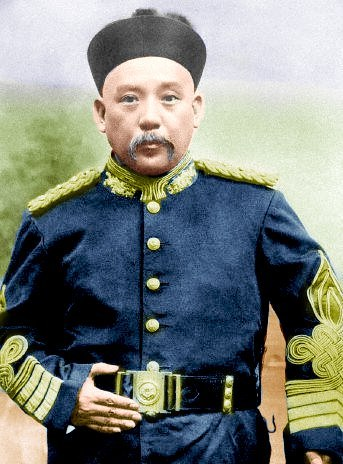
\includegraphics[scale=0.4]{Glava3/N47wYPEMph0.jpg}
	%	\label{fig:scipion} % Unique label used for referencing the figure in-text\end{document}
	%	%\addcontentsline{toc}{figure}{Figure \ref{fig:placeholder}} % Uncomment to add the figure to the table of contents%----------------------------------------------------------------------------------------
	\caption{Юань Шикай}%	CHAPTER 2
\end{figure}
Никогда и никого не побеждавший на поле брани (во время восстания Боксёров он даже целенаправленно увёл подчинённые ему части Бэйянской армии, чтобы она, избежав потерь, продолжала играть роль важного фактора китайской политики), он был весьма искусным интриганом. В самом деле, нужно было быть весьма талантливым, гуттаперчевым человеком, чтобы стать как последним первым министром Империи Цин (2 ноября 1911 — 10 марта 1912), так и первым президентом Китайской Республики – при том, что большая часть революционеров-синьхайцев откровенно ненавидела Шикая, но вот поделать с ним ничего не могла, так как именно он был той точкой, осью, которая согласовывала интересы новых властей и старых силовиков и хоть как то позволяла держать последних в узде. С Юань Шикаем японцам было бы довольно удобно иметь дело – вот только, что гораздо важнее, они были не единственными участниками игры. С апреля по август 1912 года Юань Шикай получал от различных западных держав по 6 миллионов юаней ежемесячного в счёт будущего «реорганизационного займа»; эти деньги шли на укрепление Бэйянской армии, на подкуп колеблющихся республиканцев (особенно командного состава войск, концентрировавшихся на юге страны, где республиканские настроения преобладали), политиков и депутатов парламента. Наращивая мощь по прежнему верной ему Бэйянской армии, Юань Шикай последовательно сокращал численность республиканских войск Юга, и к марту 1913 года вооружённые силы провинций Цзянсу, Аньхой, Цзянси, Хунань и Сычуань потеряли 16 дивизий. Лидеры левых республиканцев не возражали против расформирования войск, набранных из необученных добровольцев в период борьбы против династии Цин, так как полагали, что, пожертвовав этим «балластом», можно будет сохранить все старые кадровые войска Наньянской армии. Однако Юань Шикай в середине 1912 года лишил Хуан Сина должности командующего войсками Юга, разрушив военную структуру левых республиканцев. В целом президент вёл себя жёстко и реалистично, а левые республиканцы зачастую действовали так, словно Китай уже стал страной буржуазной законности и порядка. Вообще, хотя, конечно, и с очень большими натяжками, можно увидеть параллели между этим периодом китайской истории и отечественными событиями 1993 года. Исход борьбы между парламентом, где доминировал Гоминьдан, и президентом, опиравшимся на верные ему части армии, во всяком случае, был очень похожим. Юань Шикай сделался пожизненным президентом, а в 1915 он попытается даже стать императором, для чего организовали специальный референдум (разумеется, срежессированный). Необходимые голоса президент получил, но вот поддержкой военных на сей раз заручиться не смог – самого хитреца Шикая готовы были терпеть, но это не распространялось на его потомков. Дни монархии в Поднебесной были сочтены. Что до Сунь Ятсена, лидера революционеров, то ему в 1913 пришлось бежать из страны. Ирония судьбы в том, что местом назначения вновь стала Япония, хотя она была одной из тех сил, что ставили на Шикая.

Однако, оставим ненадолго китайскую тему, потому что на календаре появилась роковая дата 28 июня 1914 – день Сараевского убийства. Поначалу, Японии почти не было дела до того кризиса, который постепенно нарастал в Европе, хотя, конечно, совсем не замечать и не учитывать его она не могла. Но вот 1 августа 1914 то, что раньше было лишь схваткой Австро-Венгрии и Сербии, превращается в войну Германии против России, а значит Центральных держав против Антанты. Что это означало для японцев? Начать стоит с того, что к 1914 году существовал формальный и обоюдовыгодный, прошедший проверку временем англо-японский союз (подробнее о нём мы ещё поговорим далее). Выходит, всё просто – союзнические обязательства предписывали Империи Восходящего солнца вступление в войну? Вовсе нет. Во-первых, договор был оборонительным, а Британия 4 августа 1914, пусть и в ответ на агрессию в отношении нейтральной Бельгии, сама объявила войну Германской Империи. Во-вторых, сферой действия союза была исключительно Азия: нормы договора предусматривали общие и специальные интересы англичан и японцев. Общие интересы сводились к сохранению мира в областях восточной Азии и Индии, к обеспечению независимости и целостности Китая и к принципу равенства всех народов в торговле и промышленности в Китае. Специальные интересы у каждого союзника были различны. Специальный интерес Англии — в безопасности индийской границы. Специальный интерес Японии — в Корее, которая признавалась Англией состоящей под исключительным влиянием Японии. Наконец, в третьих, сами британцы не так чтобы горели желанием видеть Японию в числе воюющих держав, даже и на своей стороне. Британский министр иностранных дел сэр Эдуард Грей боялся, причём более чем обоснованно, что в случае участия в войне, Япония, не оказав существенной помощи союзникам (было очевидно, что своих войск в Европу, где должны были разгореться основные сражения, она не пошлёт), расширит свои владения сверх всяких пределов, а, прежде всего, достигнет преобладания в Китае. 

\begin{figure}[h!tb] 
	\centering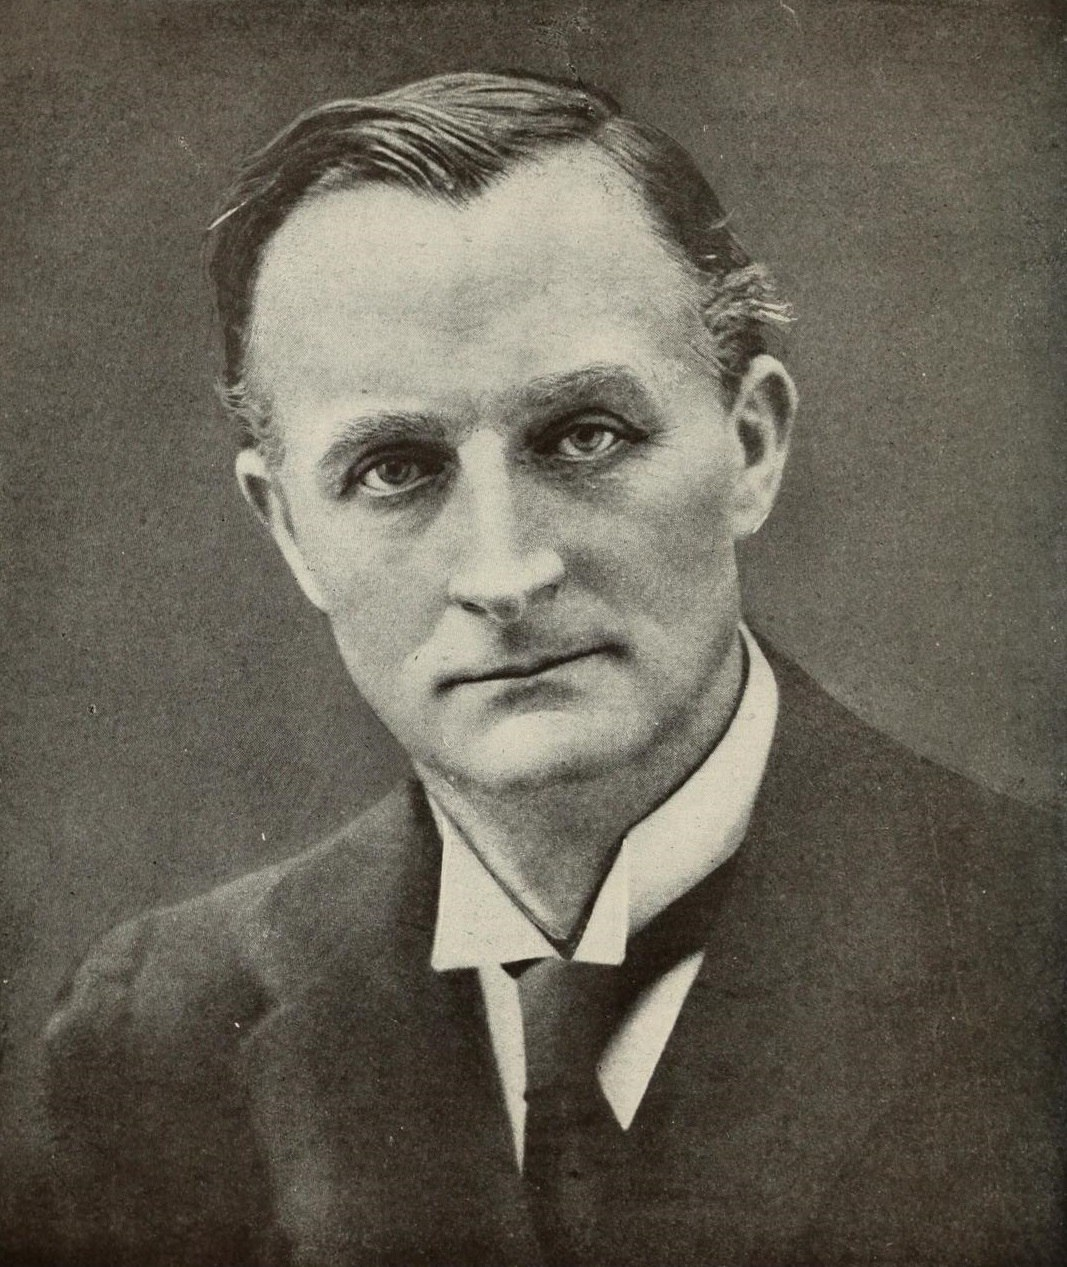
\includegraphics[scale=0.4]{Glava3/1v5GXqxlv_I.jpg}
	%	\label{fig:scipion} % Unique label used for referencing the figure in-text\end{document}
	%	%\addcontentsline{toc}{figure}{Figure \ref{fig:placeholder}} % Uncomment to add the figure to the table of contents%----------------------------------------------------------------------------------------
	\caption{Эдуард Грей, виконт Фаллодон, министр иностранных дел Великобритании в период с 10 декабря 1905 по 10 декабря 1916}%	CHAPTER 2
\end{figure}

Несмотря на все возражения Адмиралтейства, Грей пытался помешать вступлению Японии в войну. 1 августа 1914 года он прямо сообщил своему японскому коллеге Като, что Великобритании потребуется помощь только в случае атаки дальневосточных колоний. Однако усилиям Грея суждено было остаться бесплодными, потому что другой влиятельный британский политик полагал, что сражающаяся Япония будет полезна Британской империи. Этим политиком был никто иной, как сэр Уинстон Черчилль, занимавший в ту пору пост Первого лорда Адмиралтейства. В этом качестве он обязан был решить непростую проблему: при всей мощи Королевского флота, его сил на то, чтобы одновременно надёжно блокировать немецкий Флот Открытого моря, гарантируя победу над ним в случае попытки прорыва, и на то, чтобы при этом иметь значимые эскадры в дальних морях и колониях очевидно не хватало. Черчилль избрал по-видимому верный путь концентрации и сосредоточения на основном противнике. Таким образом, в связи с тем, что все британские дредноуты были сосредоточены в Европе, на Тихом океане, да даже и в Индийском тоже, остались только сравнительно старые тяжёлые корабли. Отстаивая правильность такого расположения сил, Черчилль ещё в марте 1914 года во время выступления в палате общин заявил, что поражение главных сил британского флота в Европе сделает маленькую эскадру на Тихом океане беспомощной. Любая британская эскадра в этом районе неизбежно будет уступать главным силам флота европейских противников: "…два или три дредноута в австралийских водах будут бесполезны после поражения британского флота в отечественных водах".

Как следствие этого, Черчилль опасался, что подчёркнутый отказ от помощи японцев вызовет их раздражение и недоверие, а нехватка собственных сил на удалённых ТВД может привести к такому нежелательному исходу, как самостоятельная экспансия Империи Восходящего солнца, вне связи с Британией и её, пусть даже косвенного, контроля. Наконец, в самом худшем случае, существовал риск, хотя и очень скромный, но совсем игнорировать его британцы не могли, что Япония вообще будет сражаться на стороне Германии. 11 августа 1914 года Черчилль, опасаясь, что Грей всё-таки выступит против участия Японии в войне или постарается ограничить такое участие, заявил ему: "Я думаю, что вы можете окончательно расхолодить их. Я не вижу середины между их участием и неучастием. Если они вступят в войну, мы должны приветствовать их как товарищей. Ваша последняя телеграмма в Японию почти враждебна. Я боюсь, что просто не понимаю хода ваших мыслей, и в этом аспекте не могу следовать вашим намерениям. Эта телеграмма заставляет меня трепетать. Мы все составляем единое целое, и я хотел бы оказывать всемерную поддержку вашей политике. Но я категорически возражаю против препятствий японцам. Вы легко можете нанести смертельный удар нашим отношениям, последствия которого будут ощущаться ещё слишком долго. Шторм вот-вот разразится".

Сложно сказать, насколько на позицию министра иностранных дел повлиял именно этот разговор, но, в конечном итоге, Грей примирился с перспективой увидеть в ближайшее время воюющую Японию.

Но что же сами японцы? Японская империя, как кажется, была совершенно вольна выбирать. Фактически же выбор был между вступление в войну на стороне Антанты, или нейтралитетом. Почему именно так? Отчего не рассматривается вариант с войной на стороне Германии? А ведь именно на подобный поворот событий надеялись (хотя на самом деле совершенно утопически) довольно много людей в Берлине, вплоть до самого кайзера – что японцы решат ударить в спину России, скованной боями на Западе. Ведь в Русско-японскую войну Страна Восходящего солнца одержала победу. Что мешало теперь, при жестоко связанной в Европе России предпринять новое наступление?

Во-первых, хотя это на первый взгляд и прозвучит парадоксально, именно война 1904-1905 и опыт победы в ней. При том, что успех Японии на фронтах, и, особенно, на морях был бесспорным, заключённый по итогам боевых действий Портсмутский мир был, мягко говоря, далеко не таким, каким его хотели бы видеть и элиты, и народные массы Японии. Настолько, что это даже привело к волнениям в Токио, да таким, что в ходе их подавления погибло 17 человек, а протестующие в свою очередь разгромили до 70\% всех полицейских сооружений столицы. 
\begin{figure}[h!tb] 
	\centering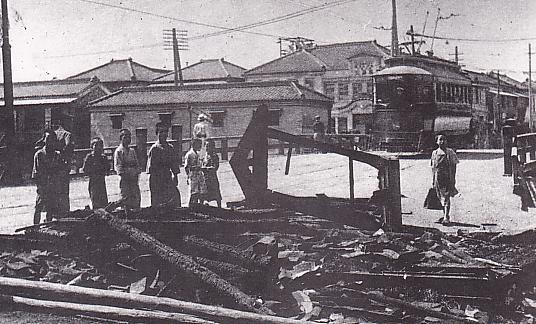
\includegraphics[scale=0.4]{Glava3/sZ8FMZJE-O0.jpg}
	%	\label{fig:scipion} % Unique label used for referencing the figure in-text\end{document}
	%	%\addcontentsline{toc}{figure}{Figure \ref{fig:placeholder}} % Uncomment to add the figure to the table of contents%----------------------------------------------------------------------------------------
	\caption{Последствия возмущений в Токио}%	CHAPTER 2
\end{figure}

Половина Сахалина, права на Южноманчжурскую железную дорогу, передача Ляодунского полуострова (при этом формально по прежнему китайского - переходили от владельца к владельцу лишь арендные права) - и ни единой монеты или банкноты контрибуции. Да, в известной степени такой результат переговоров объясняется дипломатическими талантами и ловкостью премьер-министра Российской Империи Витте — "графа Полусахалинского", но, конечно, не только. Сущностной причиной было истощение Японии войной. Потери, составлявшие по разным данным от 49 до 80 тысяч человек, конечно, были не столь велики, чтобы поставить под сомнение возможность империи сражаться дальше. Но, кроме человеческих ресурсов, есть ещё экономика, есть финансы - и вот там всё было очень серьёзно и мрачно. За время войны внешний долг России возрос на треть, что, конечно, довольно много, но это ни в какое сравнение не идёт с тем, что произошло в Японии, где внешний долг увеличился четырёхкратно, достигнув совершенно астрономической с поправкой на эпоху суммы в 2 400 000 000 иен.

Кроме того, было не очень ясно как и за счёт чего Япония могла бы принудить Российскую Империю к миру на своих условиях. Наступать от Мукдена до севера Манчжурии? Переходить границу с Сибирью? Даже если эти, уже весьма утопичные с точки зрения военной логистики планы были бы реализованы, то, не говоря уже о том, что на это ушли бы новые десятки тысяч жизней и сотни миллионов иен, это всё равно и близко не создавало такой фатальной угрозы для России, которая заставила бы её капитулировать перед японскими требованиями (например, о передаче всего Приморья). Скорее даже наоборот. Руководство Империи Восходящего солнца оказалось достаточно мудрым, чтобы понять это в 1905, но сильно слаще от этого горькая пилюля победы без плодов не становилась. В итоге Портсмут принес Японии, помимо резкого взлёта престижа (что оказалось едва ли не самым важным из последствий её успеха), и безопасности уже имевшихся приобретений (а именно Кореи, которая была формально аннексирована в 1910), такие территориальные и хозяйственные активы, которые без больших денежных вливаний могли принести хоть какую-то пользу только в весьма отдалённой перспективе. А вот денег как раз и не было.

К 1914 году стратегически здесь не поменялось ничего. Даже то, что у России появился другой, по определению основной фронт в Европе, на самом деле меняло картину не так сильно, как можно бы было подумать. Во-первых, и в 1904-1905, даже на конечной стадии войны, в период битвы при Мукдене численно основная часть армии Российской Империи находилась отнюдь не на Дальнем Востоке. Во-вторых, чего, конечно, японцы знать не могли, но тем не менее, основной удар Германии в начале войны в полном соответствии с Планом Шлиффена направлялся на Францию, так что в течение большей части 1914 не столько Россия была скованна, сколько Австро-Венгрия с большим трудом пыталась сковать Россию. Даже победа Гинденбурга под Танненбергом лишь частично изменила положение дел, но ещё отнюдь не перевернула доску. Только 1915 год, когда Германия решила перенести свой основной удар на Восток, станет критическим для Российской Империи.

Да, повторю, этого, конечно, японцы не знали. Для них всё сводилось к двум вопросам. Первый: будут ли переброшены на запад Сибирские стрелковые корпуса и, если да, то в какой срок? И второй - даже если да, то, всё равно, какой план кампании избрать? И тут мы возвращаемся к тому, о чём говорилось выше - совершенно непонятно, как именно бить по России так, чтобы ей стало действительно больно? Предположим, японцы смогли бы высадить крупный экспедиционный корпус в Манчжурии и, продвигаясь вдоль ж/д линии - а других коммуникаций там просто нет, дойти до Амура. К этому времени они в полной мере - и даже с превышением испытали бы на себе всё, что испытывала наша армия в Русско-японскую, вися на тонкой ниточке Транссиба (пропускная способность которого к 1914, к слову, напротив, возросла). Что дальше? Форсировать Амур? Идти на Благовещенск? На Романов-на-Амуре? На Хабаровск? Условия Дальнего Востока и Сибири были бы просто идеальны для реализации "скифской тактики" заманивания и перерезания линий снабжения, которое и без того было бы затруднено до крайности. Япония - остров а значит всякое обеспечение экспедиционных сил обязано изначально базироваться на суда. В 1904-1905 задачу удалось решить во многом потому, что время в пути от японских портов до Кореи, откуда грузы доставлялись в войска, занимал вместе с погрузкой и разгрузкой порядка суток. Скорость компенсировала недостаток грузоподъёмности. Но теперь вообразим, что группировка в 300-400 тысяч человек находится не у Мукдена, а у Амура...

Наконец, сама масштабная мобилизация была слишком дорогим удовольствием. Япония не была готова и не желала крупномасштабной войны с многочисленными полевыми армиями. Не желала затевать авантюру в отношении России. Не желала порывать с Англией, чья морская слабость на Востоке явно была явлением сугубо временным. Корабли, как ушли, так могли потом и вернуться. А вот уничтожить основу - порты, инфраструктуру, морские базы... нет, пока ещё никто в Японии не решался даже помыслить о войне с Владычицей морей. Положим, взять Гонконг было бы не так трудно, но он находился бы под постоянной угрозой контрудара, пока Британия владела Сингапуром. Этот стратегически важный пункт, "Гибралтар Азии" был первоклассной морской крепостью. Даже во время Второй мировой войны его сравнительно лёгкое взятие, кроме ошибок и легкомысленности руководителей обороны было обусловлено сочетанием таких факторов, на которые в 1910-е, даже и в период ПМВ японцы не могли рассчитывать. В 1940, пользуясь разгромом французов в Европе, они без кровопролития подчинили себе принадлежавшую им часть Индокитая, чем, в свою очередь, смогли решительно склонить к союзу Тайланд. Это сделало реальным удар по Сингапуру с суши. Это и большой технический прогресс авиации.

А в 1914 у Японии, это тоже стоит отметить, имелось лишь 2 дредноута: Кавати и Сэтцу. Оба – достаточно сильно уступающие новейшим кораблям Германии, США и, конечно, Англии. Их главный калибр, представленный 305-мм орудиями, во-первых был так расположен на кораблях, что сосредоточенный огонь по одной цели могли вести только 8 орудий. Во-вторых сами эти орудия имели при общем калибре разную длину стволов, а значит – разную баллистику, что во многом ставило под сомнение всю концепцию линкоров-дредноутов all big guns, так как они с большим трудом могли вести единую залповую стрельбу. Собственно, вообще половина ГК линкоров была японского производства, а половина – поставлена фирмой Армстронг из Англии.

\begin{figure}[h!tb] 
	\centering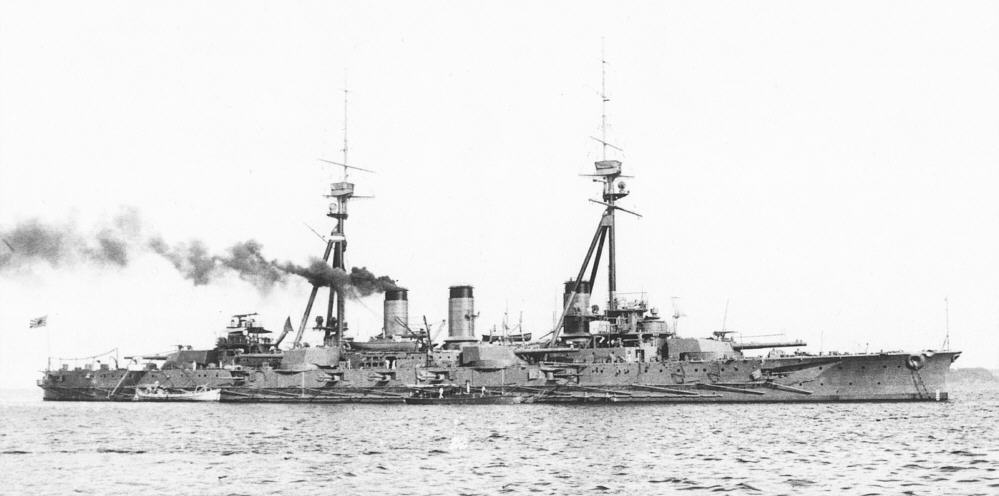
\includegraphics[scale=0.4]{Glava3/sbSwXbGYo1g.jpg}
	%	\label{fig:scipion} % Unique label used for referencing the figure in-text\end{document}
	%	%\addcontentsline{toc}{figure}{Figure \ref{fig:placeholder}} % Uncomment to add the figure to the table of contents%----------------------------------------------------------------------------------------
	\caption{Линкор Сэтцу — один из двух первых японских дредноутов}%	CHAPTER 2
\end{figure}

Да, довольно много линкоров и линейных крейсеров находилось на стапелях. Новые линкоры – Фусо и Ямасиро, заложенные в 1912 году, будут достроены только 5 лет спустя – в 1917. Линейные крейсера типа Конго: Конго, Хиэй, Кирисима и Харуна при закладке в 1911-1912 годах строились быстрее. Собственно, Конго был готов уже в августе 1913, а Хиэй достраивали в августе 1914, но всё равно это не шло ни в какое сравнение с 20 дредноутами и 9 линейными крейсерами Британии (это не считая рядка кораблей, которые были достроены в самом скором времени после августа 1914, а также реквизированных судов, строившихся для флотов третьих стран). Япония весьма успешно переходила от использования спущенных за границей судов (к слову, по преимуществу именно в Англии– все японские броненосцы – участники Цусимского боя строились на верфях Альбиона) к собственной их постройке. Верфи Йокосуки и Куре стремительно совершенствовались и могли выпускать всё более крупные и мощные линкоры, даже крупные их серии, но вот темпы строительства пока оставляли желать лучшего. Если Конго и остальные ещё укладывались в разумные пределы, то по 5 лет на Фусо и Ямасиро – это, конечно, много. Уже скоро японцы добьются больших успехов и здесь, но для этого должно было пройти ещё некоторое время от 1914.

\begin{figure}[h!tb] 
	\centering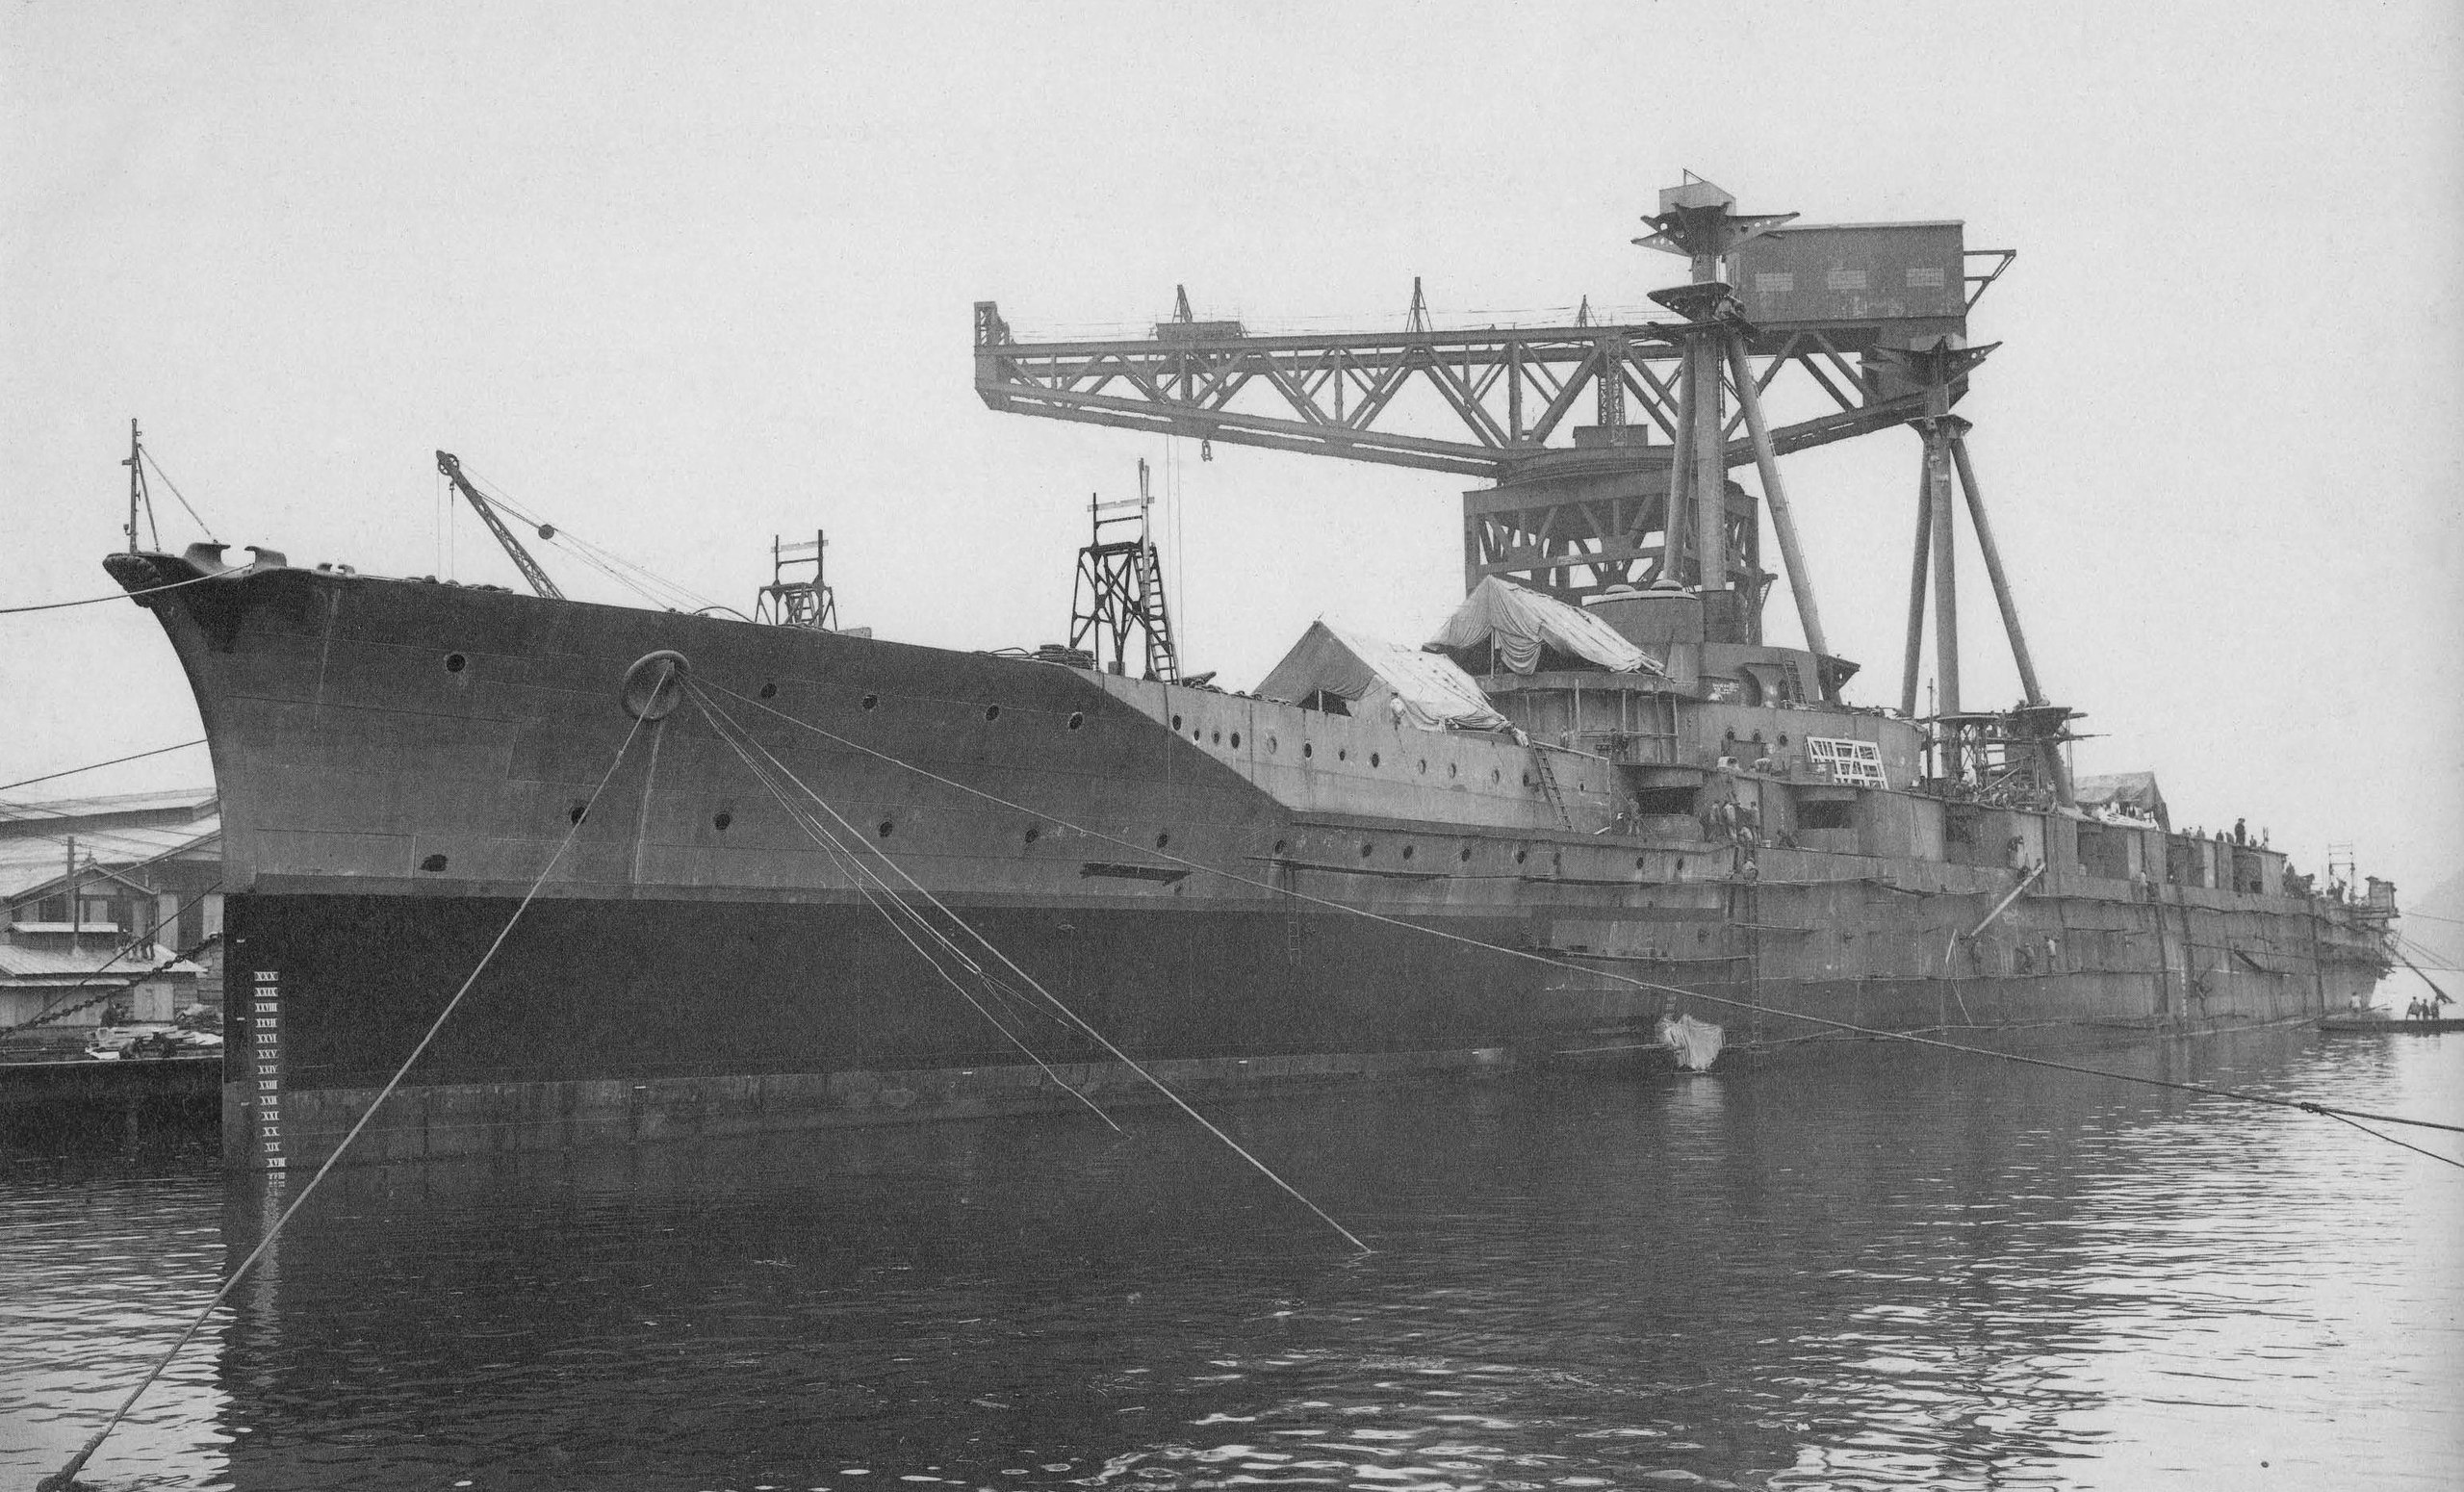
\includegraphics[scale=0.2]{Glava3/JWJxkm_fvXQ.jpg}
	%	\label{fig:scipion} % Unique label used for referencing the figure in-text\end{document}
	%	%\addcontentsline{toc}{figure}{Figure \ref{fig:placeholder}} % Uncomment to add the figure to the table of contents%----------------------------------------------------------------------------------------
	\caption{Линейный крейсер Хиэй на стапеле в Йокосуке}%	CHAPTER 2
\end{figure}

Итак, война на стороне Центральных держав обещала Японии много рисков, много затрат и очень сомнительные бенефиции, а потому, в общем, и не рассматривалась. Нейтралитет или Антанта? У нейтрального статуса, без сомнения, было немало плюсов. Первый, наиболее очевидный – отсутствие прямых и косвенных военных затрат. Второй, тоже достаточно понятный – возможность с выгодой торговать с обеими сторонами конфликта, вынужденными разорвать свои прежние контакты и связи. Конечно, те же англичане едва ли позволили бы пройти кораблям с военными грузами в порты Германии, но всё равно статус нейтрального государства дал бы японцам довольно много возможностей для извлечения материальной выгоды. Наконец, та и другая воюющая сторона вполне могли последовательно идти в отношении Японии на известные уступки, лишь бы она не присоединилась к противной стороне. К слову, японский ультиматум Германской империи, о котором будет сказано чуть ниже, формально не закрывал двери именно для такого варианта. К плюсам нейтралитета можно, без сомнений, отнести и большую степень контроля над собственным обществом. Внутренний порядок и покой были особенно ценны для Империи Восходящего солнца в условиях, когда на место Мэйдзи приходил малахольный Тайсё. Тут уместно будет вспомнить, что объявление войны Германии, а оно состоялось 15 августа 1914, даже формально произошло в период междуцарствия – в трёхлетний "траур" по умершему Муцухито, когда его сын, хоть и объявленный императором, короны не получил. О реальном правлении болезного в 1914 тем паче говорить не приходится. И, при всём этом, решительно каждый шаг Японии делается именно от императорского имени, так что проследить кто именно принимал принципиальное решение весьма непросто. Судя по всему, в августе 1914 это всё ещё были Гэнро, но уже совместно и при немалом влиянии армии. Армии, которая твёрдо считала, что её аргумент перевешивает все блага мира. И этим аргументом был Китай. Империя Восходящего солнца вступила в Первую мировую не против Германии и даже не за Антанту. Она сражалась в ней за господство в Китае и использовала её как предлог, чтобы наводнить его войсками.

Ну а теперь – всё по порядку. Трудно сказать, решились ли японцы на войну ещё до того, как Грей в Англии переменил под влиянием ещё довольно молодого и горячего сэра Уинстона своё мнение, или уже после. Мне представляется, что в основном стратегия действий страны в условиях мировой бури была определена в промежутке от 4 (вступление в ПМВ Британской империи) до 10 августа. 15 числа японское правительство (по букве – лично император) выдвинули немцам ультиматум следующего содержания: японцы требовали отзыва германских войск с Тихого океана, в том числе вывода кораблей с базы Циндао, взрыва укреплений порта и передачи Японии арендуемой Германской империей территории на Шаньдунском полуострове Китая. Японцы также потребовали передачи им германских тихоокеанских колоний (не очень ясно, временной – до окончания войны, или постоянной). Нельзя исключать, что в Берлине, обдумав и взвесив всё, сочли бы за благо согласиться на эти условия – достаточно унизительные, но, в общем, не особенно обременительные. Японцы требовали только то, что Германия и так не могла бы удержать. Это был последний шанс сохранить Страну Восходящего солнца нейтральной. Но медлительность и низкий профессиональный уровень немецкой кайзеровской дипломатии вновь дал себя знать. Решать и действовать нужно было немедленно, а Берлин тянул. В течение недели ответа не последовало, и тогда Япония 23 августа 1914 года императорским манифестом объявила войну Германии. Манифест гласил:

"С возникновением настоящей войны в Европе, на бедственные последствия которой мы взираем с великим прискорбием, мы, со своей стороны, питали надежду сохранить мир на Дальнем Востоке, соблюдая строгий нейтралитет. Но Германия принимает в Цзяо-Чжоу спешные военные приготовления, а её вооружённые корабли, крейсирующие в водах Восточной Азии, угрожают нашей торговле и торговле нашей союзницы.

И вот с глубокой скорбью мы, невзирая на нашу преданность делу мира, были вынуждены объявить войну… Мы глубоко желаем, чтобы благодаря преданности, долгу и отваге наших верных подданных мир был в скором времени восстановлен и воссияла слава империи.

…Сим мы объявляем войну Германии и повелеваем нашим армии и флоту открыть военные действия против сей Империи, со всей мощью…"

В действительности, однако, о "всей мощи" не было и речи. Япония стремилась действовать быстро, четко, но экономно – и, в общем, это ей удалось. Прежде всего, конечно, по той простой причине, что немецкие силы в регионе Тихого океана были таковы, что вопрос стоял не о том, как они могли бы отразить удары врага, а о том, как быстро они будут уничтожены, и покроют ли они себя при этом славой, или позором. На немецких островах, таких как Германское Самоа, Германская Новая Гвинея, или Германская Микронезия, сопротивление оказывать было попросту некому, так что борьба шла не между немцами и странами Антанты, а между Японией и Британскими доминионами – Австралией и Новой Зеландией на предмет того, кто быстрее их займёт. 

\begin{figure}[h!tb] 
	\centering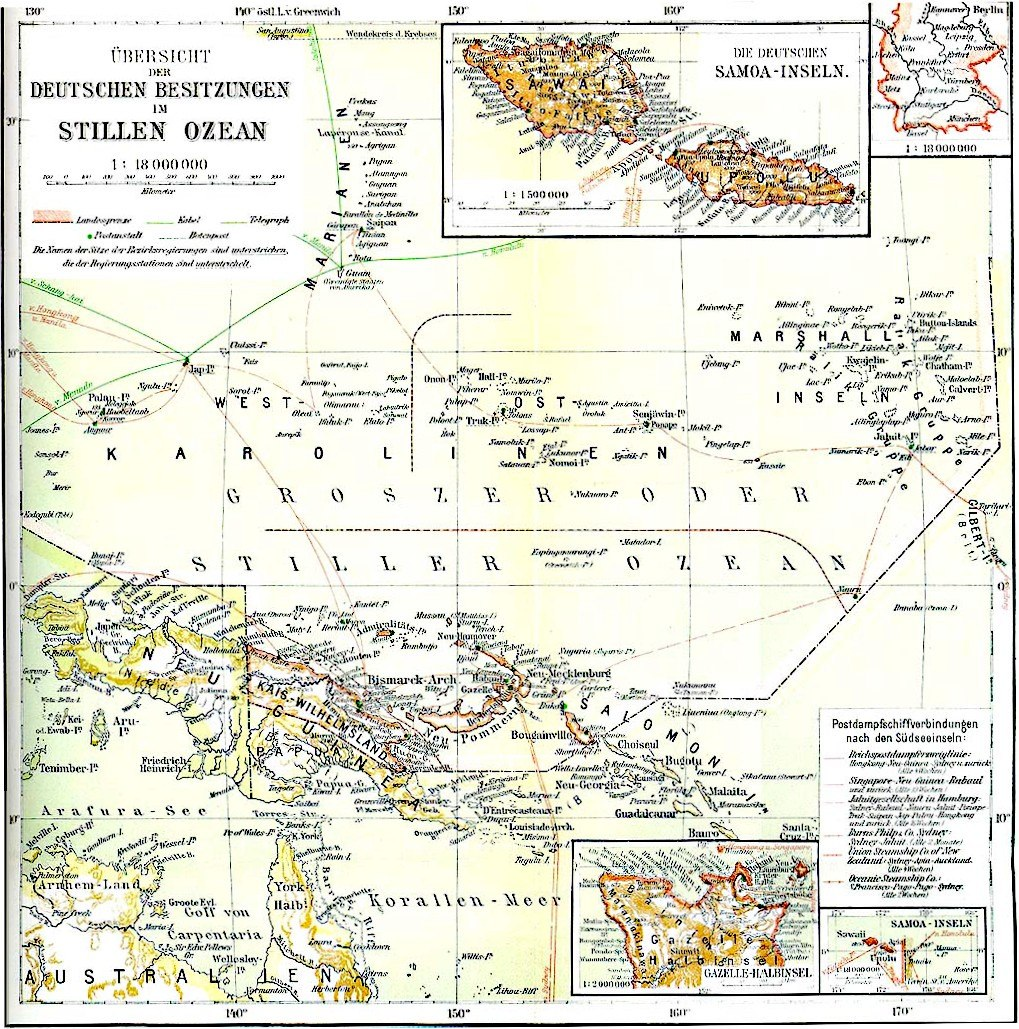
\includegraphics[scale=0.4]{Glava3/Ws5-lBsrvxc.jpg}
	%	\label{fig:scipion} % Unique label used for referencing the figure in-text\end{document}
	%	%\addcontentsline{toc}{figure}{Figure \ref{fig:placeholder}} % Uncomment to add the figure to the table of contents%----------------------------------------------------------------------------------------
	\caption{Немецкие владения в Тихом океане}%	CHAPTER 2
\end{figure}

На Самоа и Новую Гвинею ввиду географической близости первыми успели Новозеландцы и Австралийцы соответственно. Последним противодействовали 61 немец и 240 местных вспомогательных полицейских. Дело было сделано в несколько дней – и так оно, примерно, происходило везде. Если говорить о флоте, то вся «Австралийская станция», ответственная за демонстрацию германского флага в Южных морях, состояла из одной канонерки «Гайер», которая на момент начала Первой мировой войны находилась с визитом в голландских водах.

Японцы тоже не теряли времени: 1-я эскадра Южного моря под командованием вице-адмирала Ямая захватила атолл Джалуит, а 12 октября появилась в гавани Трука. 1 октября 2-я эскадра Южного моря контр-адмирала Мацумуры захватила принадлежащий Германии порт Рабаул на острове Новая Британия (тогда Новая Поммерания), а 7 октября прибыла на остров Яп, где встретила германскую канонерку «Планет», поспешно затопленную экипажем при виде японцев. На этом в Тихом океане всё, в общем, и окончилось, если не считать эпопеи адмирала Максимилиана фон Шпее (да, именно в его честь был назван знаменитый немецкий “карманный линкор» уже времён Второй мировой), которого искали и преследовали по всем параллелям и мередианам и который, тем не менее, едва не сумел ускользнуть, плюс дал весьма достойное сражение британцам у побережья Чили вблизи города Коронель. Но даже Шпее при всей его отчаянной храбрости задерживаться в тихоокеанских водах не планировал. К концу 1914 года японское и британское правительства с трудом урегулировали вопрос о захвате германских владений на Тихом океане. Чтобы избежать новых инцидентов, англичане согласились, что войска Британского содружества не будут действовать севернее экватора, а Марианские, Каролинские и Маршалловы острова останутся у японцев. Окончательное разграничение произошло после окончания войны.

Основное же внимание Японии, конечно, было приковано к Циндао. Здесь уместно будет сказать об этой немецкой базе несколько слов. Причин у её появления было три. Первая – чисто военная. До подписания договора об аренде 1897 года любые немецкие морские силы, находящиеся в Тихом океане, фатально зависели от портов и доков или Британии (Гонконг, Сингапур), или союзной ей Японии. Вторая – стремление “засунуть палец” в китайский пирог. Без некоего опорного пункта на его территории резко уменьшалась скорость возможной реакции Германии на ущемление своих интересов в Поднебесной. Понятно, что для любой полновесной акции устрашения или возмездия всё равно потребовалось бы привлечение каких-то экспедиционных сил из метрополии (как это в итоге случалось в ходе восстания Ихэтуаней), но, как правило, было достаточно лишь демонстрации присутствия. Ну а главное – немцы нуждались в своём свободном порте для выгрузки и складирования поставляемых в Китай товаров. Тирпц в своих мемуарах пишет об этом так: “Если германские купцы хотели перестать быть посредниками между англичанами и китайцами и бросить на азиатские рынки немецкие товары, то они нуждались в собственном Гонконге…” Спорить с этим было трудно. Вообще в 1890-е стремительно разворачивалось глобальная конкуренция, в итоге вылившаяся в противостояние, между промышленными товарами Британии и Германии, в котором при равных условиях немцы, как правило, побеждали, вот только этих условий им почти никогда не удавалось добиться.

Почему чуть выше я вспомнил про Тирпица? Потому что Циндао – это во всех смыслах его детище. Начать с того, что именно он, тогда ещё в ранге командующего Восточно-Азиатской крейсерской эскадрой, лично выбрал из нескольких вариантов то место, где должна была быть развёрнута инфраструктура планируемой базы. Причём, помимо известной удалённости от создающего угрозу и, как минимум, неудобство Гонконга, и более привычного для европейцев, менее жаркого климата северного, а не южного Китая, Тирпиц особенно подчёркивал удобство бухты и окрестностей для обороны. Сама операция (а это действительно была почти что боевая операция – противодействия самих китайцев можно было не опасаться, они тогда находились в жалком положении, но нужно было принимать во внимание позицию целого ряда держав, прежде всего, Британии, Японии и России, а она едва ли могла быть сочувственной немцам, так что пришлось сперва быстро и скрытно вводить крейсерскую эскадру в намеченный район, а потом выдерживать в состоянии боевой готовности непродолжительную, но довольно бурную дипломатическую канонаду) произошла уже в отсутствии Тирпица, которого сменил в качестве командира Восточно-Азиатской эскадры фон Дидерихс, начавший своё стремительное возвышение творец Флота Открытого моря никогда не забывал о Циндао и по-прежнему относился к нему как, во многом, к своему проекту. К числу несомненных достоинств Тирпица, помимо прочего, следует отнести его чрезвычайную энергичность, умение придать делу динамизм, причём он не только “вертелся” сам, но и весьма неплохо заставлял крутиться окружающих.

Главной проблемой немцев было время. Гонконг к моменту возникновения на столь же пустом, как у у него изначально, месте Циндао, существовал уже без малого 40 лет, так что конкурировать с ним было очень трудно. Вообще станция чуть не стала жертвой межведомственных противоречий. В развитие порта и поселения нужно было вкладывать деньги, а для всех, кто мог бы это сделать, существовали более приоритетные и срочные задачи. Флот был в самом скором времени всецело поглощён сколь масштабными, столь и дорогими кораблестроительными программами, которые в итоге вывели его на второе место в мире. Министерство по делам колоний в гораздо большей мере интересовалось обширными территориями в Восточной Африке, которые предполагалось сделать переселенческой колонией. Министерство иностранных дел не хотело тратить свои деньги на инфраструктурные проекты. В итоге колония едва не превратилась в чемодан без ручки. Спасло её от этой участи почти исключительно внимание и труды Тирпица.

В итоге, хотя возможно было и большее, немцы достигли к 1914 не так уж и мало. Население города Циндао насчитывало 60 000 человек, порт, хотя и не был ровней гонконгскому, сделался вполне приличным и современным. 

\begin{figure}[h!tb] 
	\centering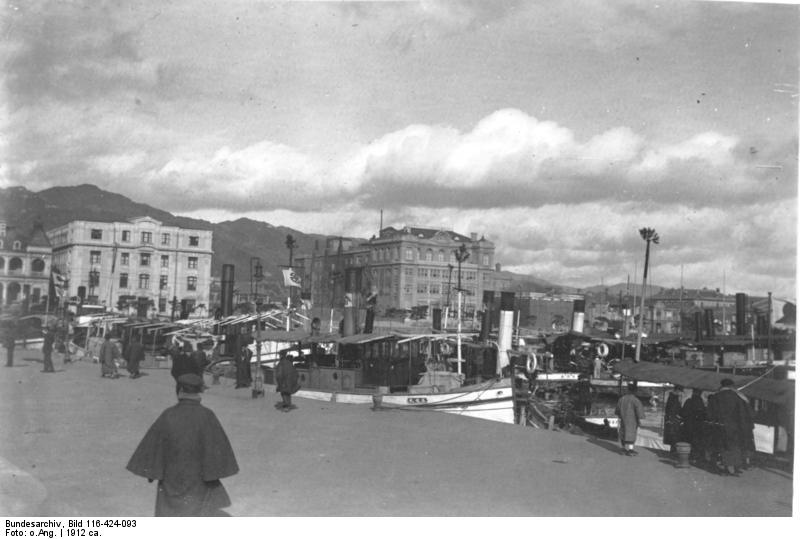
\includegraphics[scale=0.4]{Glava3/Pbn9u-W-zLI.jpg}
	%	\label{fig:scipion} % Unique label used for referencing the figure in-text\end{document}
	%	%\addcontentsline{toc}{figure}{Figure \ref{fig:placeholder}} % Uncomment to add the figure to the table of contents%----------------------------------------------------------------------------------------
	\caption{Коммерческий порт Циндао}%	CHAPTER 2
\end{figure}

Ещё важнее были экономические основы жизни колонии. Обратимся вновь к Тирпицу: “…Циндао постепенно становился тем портом, через который шла нефть с Зондских островов, имевшая большое распространение в Китае. Впрочем, быстрое развитие порта обеспечивалось уже близостью шаньдунского угля, который высоко ценится в Восточной Азии. Наличие угля в арендованной области имело первостепенное значение. К началу войны за Циндао была закреплена возможность выплавки металла из руд, добываемых в Пошане...” Иными словами, порт очень удачно встроился в хозяйственные связи, имевшиеся в регионе, и даже начал завязывать их на себе, создавать новые. Шутка ли – был намечен к постройке металлургический завод со сталеплавильными и прокатными цехами, который стал бы едва не самым крупным в Азии! Опираясь на него, немцы могли осуществить мощную интервенцию в экономику Китая, кроме того, завод позволил бы основать в самом Циндао ряд промышленных предприятий, которые использовали бы его сырьё.

Как и в целом Германию, война подрезала Циндао на взлёте. Да, город по-прежнему оставался неплохой приморской крепостью, причём защищённой не только от удара с моря, но и имеющую подготовленные позиции на суше (сложно сказать, что сыграло тут ведущую роль – немецкая ли основательность, или относительная близость Пекина, а значит и возможных китайских политических потрясений), но главная ценность его была отнюдь не военной. 


\begin{figure}[h!tb] 
	\centering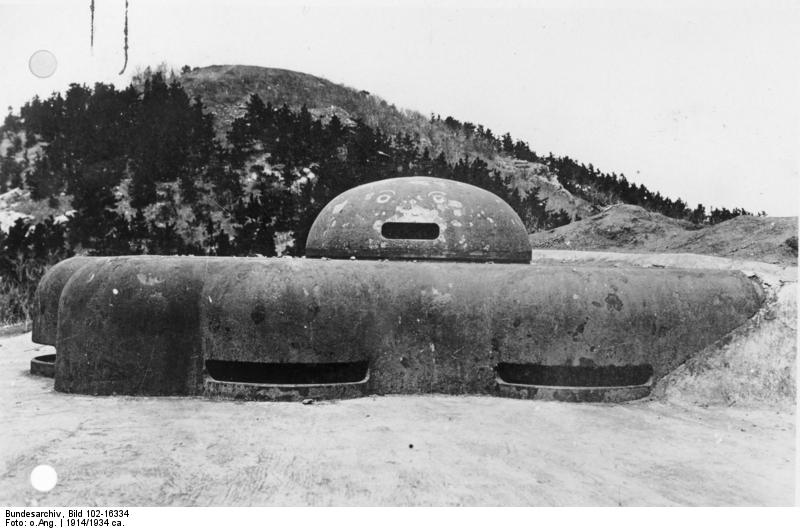
\includegraphics[scale=0.4]{Glava3/ZqmLdol8HWM.jpg}
	%	\label{fig:scipion} % Unique label used for referencing the figure in-text\end{document}
	%	%\addcontentsline{toc}{figure}{Figure \ref{fig:placeholder}} % Uncomment to add the figure to the table of contents%----------------------------------------------------------------------------------------
	\caption{Укрепления Циндао}%	CHAPTER 2
\end{figure}

Сам факт начала Первой мировой, превративший бурно развивающийся торгово-промышленный форпост одной из ведущих индустриальных держав мира в отрезанный, находящийся в глубоком стратегическом тылу у противника ощетинившийся штыками островок сопротивления, был наиболее гибельным для Циндао. Даже и безотносительно вступления в войну Японии, по всей вероятности, город пал бы. Но, конечно, вмешательство армии и флота Империи Восходящего солнца резко уменьшило сроки агонии.

Корабли японцев появились в районе Циндао очень быстро. Уже 27 августа Циндао был блокирован японской эскадрой вице-адмирала Като Садакичи. Такая оперативность объясняется не столько стремление отрезать немцев – они и так были отрезаны, сколько не дать себя обойти союзникам. В каждый момент осады Циндао японцы имели в виду прежде всего свои дальнейшие перспективы и планы в отношении Китая. Так, для взятия города был выделен экспедиционный корпус численностью свыше 30000 человек, тридцать девять военных кораблей и более пятидесяти транспортов. Англичане для содействия им выделили несколько кораблей и скорее символический отряд в 1500 человек. Немецкий гарнизон под командованием контр-адмирала Майер-Вальдека располагал 4000 бойцов, из которых существенная часть была матросами, слабо подготовленными к ведению боевых действий на суше. Тем не менее, немцам надо отдать должное – всё, что было в их силах, они сделали. Майер-Вальдек не зря отправил в день, когда стало известно о том, что японцы вступили в войну на стороне Антанты следующую телеграмму императору Вильгельму: «Остаюсь на посту до последнего». 

\begin{figure}[h!tb] 
	\centering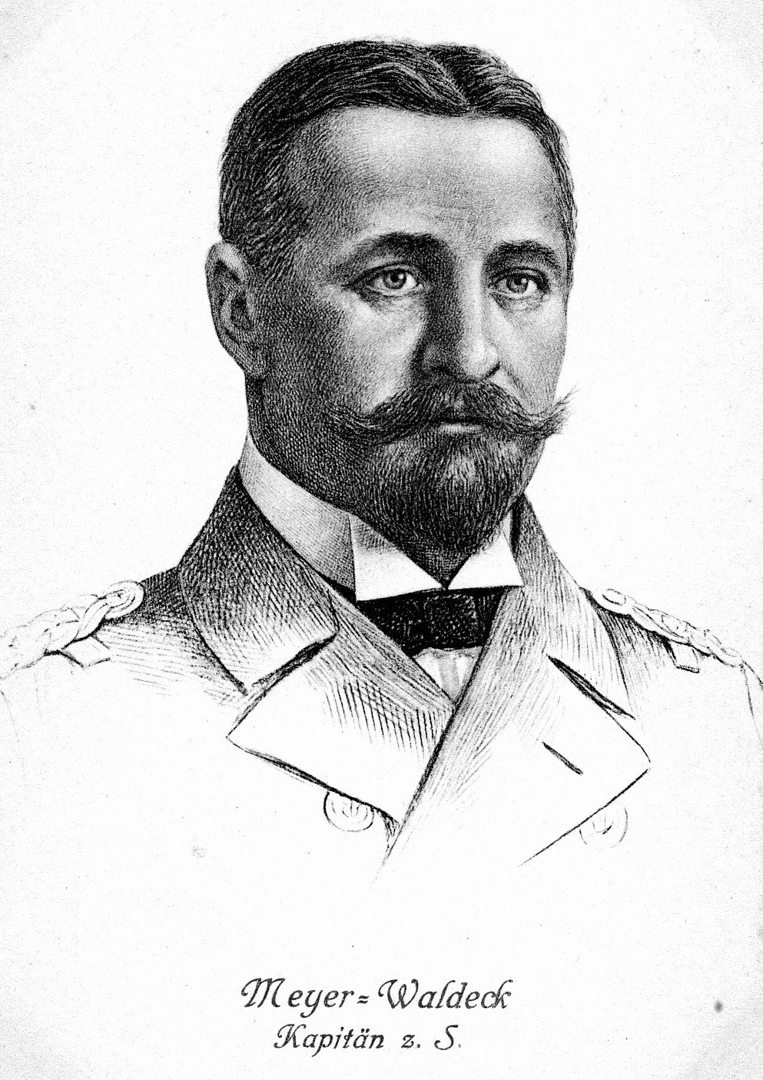
\includegraphics[scale=0.4]{Glava3/tCeondYExXg.jpg}
	%	\label{fig:scipion} % Unique label used for referencing the figure in-text\end{document}
	%	%\addcontentsline{toc}{figure}{Figure \ref{fig:placeholder}} % Uncomment to add the figure to the table of contents%----------------------------------------------------------------------------------------
	\caption{Альфред Майер-Вальдек}%	CHAPTER 2
\end{figure}

За время осады несколько японских кораблей подорвались на минах; английский броненосец «Триумф» получил повреждение от огня береговых батарей. В ночь с 17 на 18 октября немецкий миноносец S-90 под командованием капитан-лейтенанта Бруннера и вовсе сумел прорвать морскую блокаду. Ему удалось торпедировать японский крейсер «Такатихо», при этом погиб 271 человек. 

\begin{figure}[h!tb] 
	\centering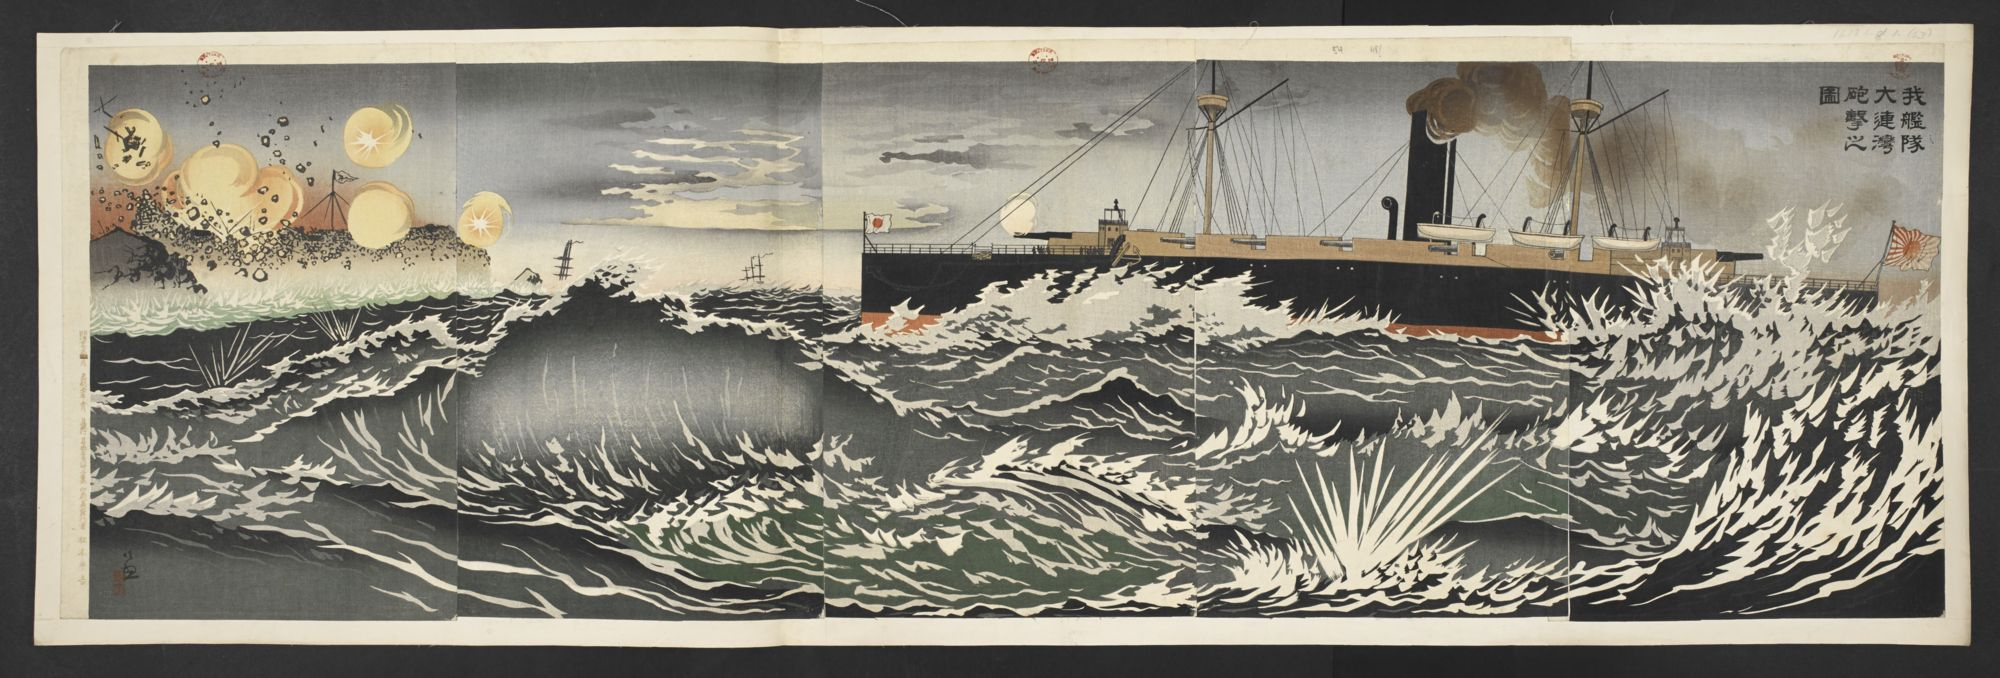
\includegraphics[scale=0.15]{Glava3/SYUEA0WTbBs.jpg}
	%	\label{fig:scipion} % Unique label used for referencing the figure in-text\end{document}
	%	%\addcontentsline{toc}{figure}{Figure \ref{fig:placeholder}} % Uncomment to add the figure to the table of contents%----------------------------------------------------------------------------------------
	\caption{Бронепалубный крейсер Такатихо, изображённый в момент обстрела порта Дальний в Русско-японскую войну}%	CHAPTER 2
\end{figure}

Вернуться в Циндао Бруннер уже не мог. Он планировал заправиться топливом в одном из нейтральных портов и продолжить атаковать японский флот, но из-за нехватки топлива выбросил миноносец на берег, после чего экипаж был интернирован китайскими властями.

Тем не менее, если, невзирая на совершённые подвиги, взглянуть на происходящее трезво, то обнаружится, что задействованный японцами наряд сил был явно избыточен. Уже обозначенные выше 30 000 человек получили могучий артиллерийский кулак (вплоть до тяжелых орудий, обстреливавших в 1904-1905 Порт-Артур), обильные запасы амуниции и снаряжения. В некоторых источниках это объясняется якобы имевшим место быть страхом японцев перед немцами, которых многие в армии по-прежнему воспринимали как учителей. Позвольте усомниться! После Русско-японской дрожь в коленях при виде белого человека у подданных Микадо прошла раз и навсегда, да и в принципе японцы не из робких. Главное же, даже завзятый трус не мог не заметить того, что немцы находятся в отчаянном положении. Наконец, и страх, и медлительность японцев были очень избирательными – когда им это было нужно, они прорвали первую линию обороны немцев в сентябре 1914 за 4 дня. И только потом, после этого, стали ожидать прибытия тяжёлых орудий и всего остального, чтобы начать генеральный штурм только 31 октября.

Истина в том, что японцы, конечно же, не взяли паузу более чем в месяц не из страха, а чтобы иметь формальный повод накрашивать своё присутствие, копить и демонстрировать наглядно силу. И не осаждённым немцам, а союзным англичанам, а главное – Китаю предназначались 43 500 снарядов, выпущенных сотней орудий за неделю, прошедшую от момента начала атаки и до капитуляции гарнизона 7 ноября 1914. 

\begin{figure}[h!tb] 
	\centering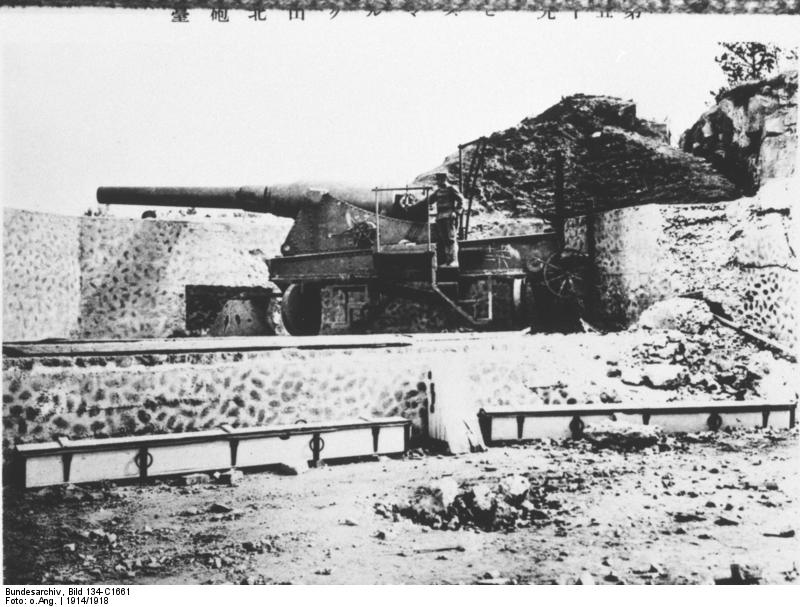
\includegraphics[scale=0.3]{Glava3/swS61nu3Jqs.jpg}
	%	\label{fig:scipion} % Unique label used for referencing the figure in-text\end{document}
	%	%\addcontentsline{toc}{figure}{Figure \ref{fig:placeholder}} % Uncomment to add the figure to the table of contents%----------------------------------------------------------------------------------------
	\caption{Форт взят. Японцы фотографируют орудия Циндао}%	CHAPTER 2
\end{figure}